\documentclass[11pt]{article}

\usepackage{titlesec}
\usepackage[hidelinks]{hyperref}
\usepackage{titling}
\usepackage[margin=1in,headheight=0pt,headsep=0pt]{geometry}
\usepackage{multicol}
\usepackage{graphicx}
\usepackage{tcolorbox}
\usepackage{multirow}
\usepackage{makecell}
\usepackage{xcolor}
\usepackage{titlesec}
\usepackage{pifont} % bullet points for itemize
\usepackage{enumitem} % packed itemize


\definecolor{mycolor}{rgb}{0.122, 0.435, 0.698}% Rule colour

% Reduce the margin from the top of the page
\setlength{\voffset}{-0.5in}
\setlength{\headsep}{5pt}


% Format some parts
\titleformat{\section}
{\Large\bfseries\uppercase}
{}
{0em}
{}[\titlerule]

\titleformat{\subsection}
{\bfseries\Large}
{$\bullet$}
{0em}
{}

\titleformat{\subsubsection}
{\bfseries}
{}
{0em}
{}

\newtcbox{\topic}{on line,
colframe=mycolor,
colback=mycolor!10!white,
boxrule=0.5pt,
arc=4pt,
boxsep=0pt,
left=6pt,
right=6pt,
top=6pt,
bottom=6pt}

\newtcbox{\nameTitleBox}{on line,
colframe=gray,
colback=white,
boxrule=1pt,
arc=2pt,
boxsep=0pt,
left=6pt,
right=6pt,
top=6pt,
bottom=6pt}

% define function
% arguments: level, place, graduation, image
\newcommand*{\eduWithDetail}[5]
{\begin{table}[h!]
	\begin{tabular*}{\textwidth}{ll@{\extracolsep{\fill}}r}
		\textbf{#1} &  #2 & \\ % \multirow{2}{*}{\includegraphics[width=40px]{#4}} \\
		#3 &  & \\
		\multicolumn{3}{l}{#5}
	\end{tabular*}
\end{table}}

\newcommand*{\eduSmall}[5]
{\begin{table}[h!]
	\begin{tabular*}{\textwidth}{ll@{\extracolsep{\fill}}r}
		\textbf{#1} &  #2 & \\ % \multirow{2}{*}{\includegraphics[width=40px]{#4}} \\
		#3 &  & \\
		\multicolumn{3}{l}{#5}
	\end{tabular*}
\end{table}}

\newcommand*{\multilineCell}[1]
{\begin{tabular}[c]{@{}l@{}} #1
\end{tabular}}

% 1: Name 2: Date 3: Lecturer 4: Level
\newcommand*{\taRecord}[4]{\textbf{#1}\quad (#3) \\ #2 \quad  #4}

\def\today{\number\day \space \ifcase\month\or
	Jan\or Feb\or Mar\or Apr\or May\or Jun\or
	Jul\or Aug\or Sep\or Oct\or Nov\or Dec\fi
	\space \number\year}


\usepackage{paracol}
\usepackage[bottom]{footmisc}
\usepackage{colortbl}
\usepackage{lipsum}
\usepackage{setspace}
\usepackage{amssymb}
\usepackage{soul}

\usepackage{hyperref}
\RequirePackage{fontawesome}

\usepackage{fontawesome}
\usepackage{setspace}

\begin{document}
	

	
% Title and Header section
% {% Image
%     \begin{minipage}[t]{100px}
%         % add a row so that contacts minipage is alligned with
%         % this line, but remove the space added for the line
%         \strut\vspace*{-\baselineskip}\newline
%         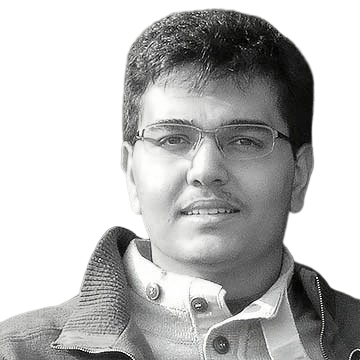
\includegraphics[width=80px]{images/farbod.png} \\
%     \end{minipage}
%     Name
%     \nameTitleBox{
%     \begin{minipage}[t]{3.5cm}
%         \vspace{8mm}
%         \noindent
%         \huge\bfseries
%         Farbod\\
%         Shahinfar
%         % \vspace{0.0cm}
%     \end{minipage}
%     }
%     \hfill\null
%     \begin{minipage}[t]{6cm}
%         \vspace{6mm}
%         % Contact Information
{ % \small
% \noindent
% \flushright
\noindent
% Phone: +989128077968 \\
\small \faEnvelope  \hspace{0.05cm}   Email: \href{mailto:iman.rahmati@sharif.edu}{iman.rahmati@sharif.edu} \space \href{mailto:imanrht@gmail.com}{imanrht@gmail.com} \\
%\faLink \hspace{0.05cm} Web page: \href{https://imanrht.github.io}{imanrht.github.io} \\
\faGithub \hspace{0.1cm} Github: \href{https://github.com/ImanRHT}{https://github.com/ImanRHT}  \\
\faLinkedin \hspace{0.1cm} Linkedin: \href{https://linkedin.com/in/iman-rahmati}{linkedin.com/in/iman-rahmati}\\
% Birthday: 25/Feb/1998 \\
}
% ===================================================================

%     \end{minipage}
% }
{\noindent \huge\bfseries Iman Rahmati}\hfill{\footnotesize updated: \today}
\vspace{-1cm}
\section{}
% Contact Information
{ % \small
% \noindent
% \flushright
\noindent
% Phone: +989128077968 \\
\small \faEnvelope  \hspace{0.05cm}   Email: \href{mailto:iman.rahmati@sharif.edu}{iman.rahmati@sharif.edu} \space \href{mailto:imanrht@gmail.com}{imanrht@gmail.com} \\
%\faLink \hspace{0.05cm} Web page: \href{https://imanrht.github.io}{imanrht.github.io} \\
\faGithub \hspace{0.1cm} Github: \href{https://github.com/ImanRHT}{https://github.com/ImanRHT}  \\
\faLinkedin \hspace{0.1cm} Linkedin: \href{https://linkedin.com/in/iman-rahmati}{linkedin.com/in/iman-rahmati}\\
% Birthday: 25/Feb/1998 \\
}
% ===================================================================
 \vspace{-2mm}

\noindent{\textbf{Research Interests:}} Distributed Systems, Mobile Edge Computing, Deep Reinforcement Learning, Federated Learning, Software Defined Networking, Performance Evaluation
\vspace{-2mm}
\section{Education}



%\vspace{-0.5cm}
%\eduWithDetail{Ph.D. Information Technology}
%{Politecnico di Milano}
%{Expected Graduation date 2026}
%{}
%{\multilineCell
%	{\hspace{5mm} \textbf{Advisor}: Prof. Gianni Antichi}
%}
\vspace{-5mm}

\eduWithDetail{MSc. Computer Software Engineering}
{\hspace{1.3cm} Sharif University of Technology (SUT)}
{Graduated Sep 2022, 17.36/20 GPA (23 units)}
{images/sharif.png}
{\multilineCell
	{
        \hspace{5mm} \textbf{Thesis Title}:
        A Novel Resource Allocation Algorithm in Edge Computing with Deep \\ \hspace{3.2cm}Reinforcement Learning \href{https://github.com/ImanRHT/Master_Thesis}{\faGithub}\\
        \hspace{5mm} \textbf{Supervisor}: Prof. Ali Movaghar \href{https://scholar.google.com/citations?user=BXNelwwAAAAJ\&hl=en}{\small \faExternalLink}}
}
\vspace{-5mm}    

\eduWithDetail{BSc. Industrial Engineering}
{\hspace{1.2cm}Khajeh Nasir Toosi University of Technology (KNTU)}
{Graduated Sep 2019}
{images/iust.png}
{%\multilineCell{\hspace{5mm}\vspace{-3mm} \\ %\textbf{Frist Rank}, 18.62/20 GPA \\
	%\hspace{5mm} \textbf{Project}:
	%Study of MMU Cache Partitioning Efficacy for Hierarchical Page Tables \\
	%\hspace{10mm} in OS Memory Management \\
	%\hspace{5mm} \textbf{Supervisor}: Dr. Mohsen Sharifi}
}
\vspace{-10mm}

% \eduSmall{High School Diploma}
% {Salam 3}
% {Graduated May 2015}
% {images/salam.png}
% {\hspace{5mm} \textbf{GPA:} 19.84/20}




\section {Publication}
I. Rahmati, H. Shah-Mansouri, A. Movaghar, \href{https://arxiv.org/pdf/2311.02525.pdf}{``QOCO: A QoE-Oriented Computation Offloading Algorithm based on Deep Reinforcement Learning for Mobile Edge Computing''}, submitted to IEEE Internet of Things Journal 2023.
\href{https://arxiv.org/pdf/2311.02525.pdf}{\small  \faExternalLink}
\href{https://github.com/ImanRHT/QOCO}{\faGithub}




\section{Academic Experience}

\large\large\textbf{Research Assistant} \vspace{-2mm}
\begin{itemize}
	\item \textbf{Research Assistant at Performance and Dependability Laboratory (PDL)} \href{https://pdl.ce.sharif.edu}{\small \faExternalLink}
	\\ Supervisor: Prof. \href{https://scholar.google.com/citations?user=BXNelwwAAAAJ\&hl=en}{Ali Movaghar} \hfill SUT, 2020-present\\
	\textbf{Research Theme:} Designed and implemented an algorithm leveraging deep reinforcement learning to optimize computation offloading decisions within mobile edge computing, with a primary focus on enhancing the Quality of Experience (QoE) for end-users of mobile applications.
\end{itemize}
\large\large\textbf{Teaching Assistant}  \vspace{-2mm}

\begin{itemize}

	\item \textbf{Performance Evaluation of Computer Systems (Head TA)} \hfill SUT, 2020-present
		\\ Prof. Ali Movaghar and Dr. Mahdi Dolati \vspace{-2mm} \href{https://scholar.google.com/citations?user=b7A2CXYAAAAJ&hl=en&oi=ao}{\small \faExternalLink}
	\item \textbf{Software Defined Networking (Head TA)} \hfill SUT, 2022
		\\ Prof. Ali Movaghar and Dr. Mohammad Hosseini \vspace{-2mm} \href{https://scholar.google.com/citations?user=iRO-DVoAAAAJ&hl=en&oi=ao}{\small \faExternalLink}
	\item \textbf{Verification of Reactive Systems} \hfill SUT, 2021
		\\ Prof. Ali Movaghar \vspace{-2mm}
	\item \textbf{Theory of Machines and Languages} \hfill SUT, 2021
		\\ Prof. Ali Movaghar \vspace{-2mm}

\end{itemize}
\large\large\textbf{Reviewer at 27th International Computer Conference} \hfill CSICC, 2022 \\
  \textcolor{white}{iiiiiii}Computer Society of Iran (CSICC) \href{http://csi.org.ir/csicc2022/index-2.html}{\small \faExternalLink}\\ \textcolor{white}{iiiiii} IEEE website published papers from this conference. \href{https://ieeexplore.ieee.org/xpl/conhome/9780464/proceeding}{\small \faExternalLink}

\section{Honors}
\begin{itemize}
	\renewcommand\labelitemi{\ding{118}}
	\item{Ranked Top 25\% in the Department of Computer Engineering among M.Sc. Students, SUT, Class 2019 \hfill Jul 2022}\vspace{-2mm}
	\item {Ranked 55$^{th}$ among 30,000 Participants in the Nationwide University Entrance Exam of Computer Engineering for M.Sc. in the Field of Software Engineering \hfill Aug 2019}\vspace{-2mm}
	\item{Ranked Top 1\% among 180,000 Participants in the Nationwide University Entrance Exam for B.Sc. in the Field of Mathematics and Physics  \hfill Jul 2014}
	\item{Achieving the 1st position in the RoboCup Competition (IranOpen)  \hfill Mar 2012}\vspace{-2mm}
\end{itemize}


\section{Academic Projects}

\begin{itemize}
	
	
		
	\item \textbf{QoE Maximization in Mobile Edge Computing} \hfill SUT, 2021\\
	Optimizing Decision-Making for Computation Offloading in Mobile Edge Computing using Deep Reinforcement Learning (Dueling Deep Q-Networks) \href{https://github.com/ImanRHT/QOCO}{\faGithub} \\
	Supervisor: Prof.  Ali Movaghar and Dr. Hamed Shah-Mansouri \href{https://scholar.google.com/citations?user=dcjIFccAAAAJ&hl=en&oi=ao}{\small \faExternalLink} 
	
	
	\item \textbf{Mobile Edge Computing Environment} \hfill SUT, 2021\\
	Modeling and Simulation of Mobile Edge Computing under Resource Constraints for Delay and Energy Optimization \href{https://github.com/ImanRHT/MEC_Environment}{\faGithub} \\
	Supervisor: Prof.  Ali Movaghar
	


	
	\item \textbf{Time Series Analysis} \hfill SUT, 2021\\
	Design a Model for forecasting Edge Server Workload using Recurrent Neural Networks such as Long Short Term Memory
	\href{https://github.com/ImanRHT/Time_Series_Prediction}{\faGithub} \\
	Supervisor: Prof.  Ali Movaghar
	
	\item \textbf{Computer Performance Evaluation} \hfill SUT, 2020\\
	Simulation and Performance Analysis of M/M/1/K Queue Model with Varied Service Orders (FCFS, Processor Sharing, Discriminatory Processor Sharing) \href{https://github.com/ImanRHT/MM1K_Queue_Simulation}{\faGithub} \\
	Supervisor: Prof.  Ali Movaghar
	


	\item \textbf{Distributed Systems} \hfill SUT, 2019\\
	A Survey on `Verification of Paxos and Raft Protocols in Distributed Consensus’ \\
	Supervisor: Dr. Mohammad Izadi	\href{https://scholar.google.com/citations?user=On8Cw-MAAAAJ&hl=en&oi=ao}{\small \faExternalLink}


%	\item \textbf{Decision Making Analysis} \hfill KNTU, 2018\\
%	A survey on ’Application of Data Envelopment Analysis (DEA) for Evaluating Efficiency by MATLAB’\\ 
%	Supervisor: Dr. Naser Safaie
%	\href{https://scholar.google.com/citations?user=J0M--CIAAAAJ&hl=en&oi=ao}{\small \faExternalLink}
	
	\item \textbf{Industrial Facilities Planning} \hfill KNTU, 2018\\
	Operational Sequence of Activities (Material Flow) and Establishment of Industrial Units in the Process of Gears Manufacturing in an Automaker Company\\
	Supervisor: Dr. Donya Rahmani
	\href{https://scholar.google.com/citations?user=qUqJT7MAAAAJ&hl=en&oi=ao}{\small \faExternalLink}
	
	\item \textbf{Project Management and Control} \hfill KNTU, 2017\\
	Scheduling, Time management and Resource Allocation in a Construction Project\\
	Supervisor: Dr. Amir Abbas Najafi
	\href{https://scholar.google.com/citations?user=adOQSIEAAAAJ&hl=en&oi=ao}{\small \faExternalLink}
	
%	\item \textbf{Quality Management} \hfill KNTU, 2017\\
%	Implementation of Failure Modes and Effects Analysis (FMEA) from a Managerial Perspective\\
%	Supervisor: Dr. Naser Safaie
	

	
\end{itemize}




\section{SELECTED COURSES}

		Theory of Distributed Systems  \hfill Computer Performance Evaluation\\
		Verification of Reactive Systems    \hspace{41.5mm} Wireless Networking \\
		Advanced Computer Networks \hspace{44.4mm}  Advanced Network Security\\
		Mobile Communications \hspace{56mm}   Computer Network Management








\section{Skills}
%\begin{itemize}[noitemsep,topsep=0pt,parsep=0pt,partopsep=0pt]
%	\item {Programming Languages: C, Python, Bash, \LaTeX}
%	\item {Frameworks \& Tools: DPDK, eBPF/XDP, AF\_XDP, Linux}
%	\item {Languages: Farsi (Native), English (Working proficiency)}
%	% \item BESS: Berkeley Extensible Software Switch
%	% \item TAS: TCP Accelartion Service
%\end{itemize}

% \subsection{Linux Programming:}
% \begin{itemize}
%     \item Linux Kernel Memory Subsystem
%     \item Developing Kernel Modules
% \end{itemize}

% \noindent \textbf{Programming Languages:}
% \begin{itemize}
%     \setlength\itemsep{0em}
%     \begin{multicols}{2}
%         \item {Python}
%         \item {C/C++}
%         \item {Javascript}
%         \item {Bash Script}
%         % \item {C\#}
%         % \item {Java}
%         % \item {SQL}
%     \end{multicols}
% \end{itemize}

% \subsection{Frameworks:}
%     \emph{React Native},
%     \emph{Flask},
%     \emph{Numpy and Matplotlib}

% \subsection{Softwares:}
% \begin{itemize}
%     \setlength\itemsep{0em}
%     \begin{multicols}{2}
%     \item{Docker}
%     \item{Git}
%     \item{PostgreSQL}
%     \item{MongoDB}
%     \item{Redis \& Memcached}
%     \item{Unity3d}
%     \item{Vim}
%     \item \LaTeX
%     \end{multicols}
% \end{itemize}

% \section {Work Experience}
% \noindent \textbf{Smart Online Monitoring Co} \par
% Mobile Application Developer \par
% January 2020 – April 2021 \par
% \begin{itemize}
%     \item Develop android application with React Native framework
%     \item Use BLE (bluetooth low energy) communication protocl
% \end{itemize}
% \topic{React Native}
% \topic{Javascript}
% \topic{BLE}
% \vspace{15pt}

% \noindent \textbf{Cognia} (DigikalaNEXT Summer Camp) \par
% Backend Developer \par
% July 2019 – March 2020 \par
% \begin{itemize}
%     \item Develop data gathering and data processing service
%     \item Deploy service with containerization
% \end{itemize}
% \topic{Python}
% \topic{Flask}
% \topic{PostgreSQL}
% \topic{Docker \& Docker Compose}
% \topic{Locust}
% \vspace{15pt}

% \noindent \textbf{Loop Game Studio} \par
% Backend Developer (A project contract) \par
% June 2019 – August 2019 \par
% \begin{itemize}
%     \item Develop a REST API server for the game.
%     \item Design a relational database for cutsomizable items in sale.
% \end{itemize}
% \topic{Python - Flask}
% \topic{PostgreSQL}
% \topic{Docker \& Docker Compose}
% \vspace{15pt}

% \noindent \textbf{ElmoGame} \par
% Game developer \par
% July 2017 – January 2019 \par
% \begin{itemize}
%     \item Work with Unity3d engine
%     \item Apply software design patterns in the project
%     \item Communicate with game server using REST APIs
% \end{itemize}
% \topic{Unity3D}
% \topic{C\#}
% \vspace{15pt}

% \section{Projects}
% \begin{multicols}{2}
% \begin{itemize}
%         \item { \emph{Footyard:} An online multi-player game developed for
%                 android devices.}
% \end{itemize}
% \end{multicols}

% \section{Languages:}
%     \emph{Persian}: Native \\
%     \emph{English}: Working Profeciency


\section{REFERENCES}

\textbf{Prof. Ali Movaghar} \href{https://scholar.google.com/citations?user=BXNelwwAAAAJ\&hl=en}{\small \faExternalLink} \hfill \href{mailto:movaghar@sharif.edu}{movaghar@sharif.edu}\\
Professor of Computer Science and Engineering Department, SUT \\
Visiting Professor of Computer Science Department, University of Michigan\\
\textbf{Dr. Hamed Shah-Mansouri} \href{https://scholar.google.com/citations?user=dcjIFccAAAAJ&hl=en&oi=ao}{\small \faExternalLink} \hfill  \href{mailto:hamedsh@sharif.edu}{hamedsh@sharif.edu}\\
Assistant Professor of Electrical Engineering Department, SUT\\
\textbf{Prof. Ali Mohammad Afshin Hemmatyar} \href{https://scholar.google.com/citations?user=wob0AskAAAAJ&hl=en&oi=ao}{\small \faExternalLink}  \hfill \href{mailto:hemmatyar@sharif.edu}{hemmatyar@sharif.edu}\\
Professor of Computer Science and Engineering Department, SUT\\
\textbf{Dr. Mahdi Dolati} \href{https://scholar.google.com/citations?user=b7A2CXYAAAAJ&hl=en&oi=ao}{\small \faExternalLink} \hfill  \href{mailto:mahdidolati@ut.ac.ir}{mahdidolati@ut.ac.ir}\\ Postdoctoral of Institute For Research In Fundamental Sciences Researcher (IPM)\\
\textbf{Dr. Mohammad Hosseini} \href{https://scholar.google.com/citations?user=iRO-DVoAAAAJ&hl=en&oi=ao}{\small \faExternalLink} \hfill  \href{mailto:hosseini@ipm.ir}{hosseini@ipm.ir} \\ Postdoctoral of Institute For Research In Fundamental Sciences Researcher (IPM)\\\\\\\\




Further information and Proofs are available upon Request.

\end{document}
